\documentclass[oneside]{diretrizes}            % Imprimir apenas frente
%\documentclass[doubleside]{diretrizes}        % Imprimir frente e verso

% Importações de pacotes
\usepackage[alf, abnt-emphasize=bf, recuo=0cm, abnt-etal-cite=2, abnt-etal-list=0]{abntex2cite}  % Citações padrão ABNT
\usepackage[utf8]{inputenc}                         % Acentuação direta
\usepackage[T1]{fontenc}                            % Codificação da fonte em 8 bits
\usepackage{graphicx}                               % Inserir figuras
\usepackage{amsfonts, amssymb, amsmath}             % Fonte e símbolos matemáticos
\usepackage{booktabs}                               % Comandos para tabelas
\usepackage{verbatim}                               % Texto é interpretado como escrito no documento
\usepackage{multirow, array}                        % Múltiplas linhas e colunas em tabelas
\usepackage{indentfirst}                            % Endenta o primeiro parágrafo de cada seção.
\usepackage{microtype}                              % Para melhorias de justificação?
\usepackage[algoruled, portuguese]{algorithm2e}     % Escrever algoritmos
\usepackage{float}                                  % Utilizado para criação de floats
\usepackage{times}                                  % Usa a fonte Times
\linespread{1.5} % espaçamento entre linhas

% Inclui o preâmbulo do documento
%
% Documento: Preâmbulo
%

\instituicao{Instituto Federal de Educação, Ciência e Tecnologia \\do Rio Grande do Sul}
\abreviatura{IFRS}
\departamento{Campus Canoas}
\local{Canoas}
\programa{Técnico em Informática Integrado ao Ensino Médio}
\nomeautor{Arthur Oliveira de Rosso}
\titulotb{GoBov - Sistema Web de Gerenciamento Bovino}
%\subtitulo{Subtítulo do trabalho}
\data{\today}
\grau{Técnico}
\dataapresentacao{DD/MM/20AA}

%Dados Orientador
\orientador{Rodrigo Perozzo Noll}
\instOrientador{IFRS}
\departamentoorientador{Campus Canoas}
\titulacaoorientador{Prof. Dr.}

%Dados Examinador 1
\nmexamum{Denise Pachman}
\instexamum{IFRS}
\departamentoexamum{Campus Restinga}
\titulacaoexamum{Prof.}

%Dados Examinador 2
\nomeexamdois{Mestre Splinter}
\instexamdois{IFRS}
\departamentoexamdois{Campus Restinga}
\titulacaoexamdois{Prof. Me.}


% Define as cores dos links e informações do PDF
\makeatletter
\hypersetup{
    portuguese,
    colorlinks,
    linkcolor=black,
    citecolor=black,
    filecolor=black,
    urlcolor=black,
    breaklinks=true,
    pdftitle={\@title},
    pdfauthor={\@author},
    pdfsubject={\imprimirpreambulo},
    pdfkeywords={abnt, latex, abntex, abntex2}
}
\makeatother

% Redefinição de labels
\renewcommand{\algorithmautorefname}{Algoritmo}
\def\equationautorefname~#1\null{Equa\c c\~ao~(#1)\null}

% Cria o índice remissivo
\makeindex

% Início do documento
\begin{document}

    % Retira espaço extra obsoleto entre as frases.
    \frenchspacing

    % Elementos pré textuais
    \pretextual
    %
% Documento: Capa
%
\author{Arthur Oliveira de Rosso}
\title{GoBov - Sistema Web de Gerenciamento Bovino.}

\makeatletter
	\begin{center}

		INSTITUTO FEDERAL DE EDUCAÇÃO, CIÊNCIA E TECNOLOGIA

		DO RIO GRANDE DO SUL

		CAMPUS CANOAS

		CURSO TÉCNICO EM INFORMÁTICA INTEGRADO AO ENSINO MÉDIO

		\vfill
		\vfill

		\@author

		\vfill

		\textbf{\@title}

		\vfill

		\textbf{Orientador:} Rodrigo Noll

		\vfill

		Canoas, \today

	\end{center}
\makeatother
              % Capa
    %
% Documento: Epígrafe
%
\thispagestyle{empty}
\begin{epigrafe}


%O fator decisivo para vencer o maior obstáculo é, invariavelmente, ultrapassar o obstáculo anterior.{\\}{\\}

\begin{autorepigrafe}
%Henry Ford
\end{autorepigrafe}

\end{epigrafe}



    %
% Documento: FOLHA DE ROSTO
%

\begin{folhaderosto}
	
    \begin{center}
    
    	\vspace*{3cm}%Espaçamento entre linhas	
		\small\expandafter\expandafter{\imprimirnomeautor}\\
		\vspace*{3cm}%Espaço entre linhas
		\normalsize\textbf{\expandafter\expandafter{\imprimirtitulotb}}\\
		
    \end{center}

    \vspace*{2cm}%Espaço entre linhas
	
	\vspace*{0.35 cm}%Espaçamento entre linhas
		    \large%tamanho da fonte 
    		\hfill%Estica horizontamente  com espaços
	    	\begin{minipage}{8 cm}%Minipagina
	    		\begin{small} %Muda tamanho da fonte
	    		\setlength{\baselineskip}{0.7\baselineskip}
				
		    	{Trabalho de Conclusão de Curso
apresentado como requisito parcial para
obtenção do grau de Técnico em
Informática pelo Instituto Federal de
Educação, Ciência e Tecnologia do Rio
Grande do Sul – Campus Canoas.}\\{ \vspace*{5cm}%Espaço entre linhas
		    	}\\{\imprimirtitulacaoorientador }{ }{\imprimirorientador}\\Orientador 
				
				
				\end{small} %Muda tamanho da fonte
		    \end{minipage}%%Minipagina
		    	
		    \vspace*{3 cm}%Espaçamento entre linhas
		    
		    \begin{center} %Alinhamento centralizado
		    	\normalsize %Muda tamanho da fonte
	    		\imprimirlocal, 
	    		\imprimirdata
	    	\end{center}%Alinhamento centralizado

\end{folhaderosto}
        % Folha de rosto
    %%
% Documento: FOLHA APROVAÇÃO
%

\makeatletter
\begin{folhadeaprovacao}

\thispagestyle{empty}%limpa estilo da pagina
	
	\begin{center}
    
		\small\textbf{\expandafter\uppercase\expandafter{\imprimirnomeautor}}\\
		\vspace*{3.0 cm}%Espaço entre linhas
		\normalsize\textbf{\expandafter\uppercase\expandafter{\imprimirtitulotb}}
		
    \end{center}
	
	\vspace*{0.35 cm}%Espaçamento entre linhas
		    \large%tamanho da fonte 
    		\hfill%Estica horizontamente  com espaços
	    	\begin{minipage}{8 cm}%Minipagina
	    		\begin{small} %Muda tamanho da fonte
	    		\setlength{\baselineskip}{0.7\baselineskip}
				
		    	{Trabalho de Conclusão de Curso apresentado como requisito parcial para obtenção do grau de
		    	{\imprimirgrau } em {\imprimirprograma } do {\imprimirinstituicao}{ - }{\imprimirabreviatura},
		    	{\imprimirdepartamento}.}\\{
		    	}\\				
				
				\end{small} %Muda tamanho da fonte
		    \end{minipage}%%Minipagina
		    	
		    \vspace*{0.6 cm}%Espaçamento entre linhas
		    
		    \large%%tamanho da fonte 
    		\hfill%%Estica horizontamente  com espaços
	    	 
		    
		    \normalsize %Muda tamanho da fonte
		    \vspace*{1.5 cm}%Espaçamento entre linhas
		    
		    \begin{minipage}{9 cm }%%Minipagina
		    {Data de Aprovação: {\imprimirdataapresentacao}}\\
		    \end{minipage}%Minipagina
			
			\begin{center}%Alinhamento centralizado
		    	\vspace*{1.21 cm}%Espaçamento entre linhas
				\textbf{Banca Examinadora}\\ %Negrito
						
				\vspace*{1 cm}%Espaçamento entre linhas
				\rule{9 cm}{.1 mm}\\
				{\imprimirtitulacaoorientador}{ }{\imprimirorientador} - {\imprimirinstOrientador} - {\imprimirdepartamentoorientador}\\
				
				Orientador\\
				
				\vspace*{1 cm}%Espaçamento entre linhas
				\rule{9 cm}{.1 mm}\\
				{\imprimirtitulacaocoorientador}{ }{\imprimircoorientador} - {\imprimirinstCoorientador} - {\imprimirdepartamentocoorientador}\\
				
				Co-Orientador\\
			
				\vspace*{1 cm}%Espaçamento entre linhas
				\rule{9 cm}{.1 mm}\\
				\imprimirtitulacaoexamum{ }\imprimirnmexamum - \imprimirinstexamum - \imprimirdepartamentoexamum\\
				Membro da Banca
				
				\vspace*{1 cm}%Espaçamento entre linhas
				\rule{9 cm}{.1 mm}\\				
								
				\imprimirtitulacaoexamdois{ }\imprimirnomeexamdois - \imprimirinstexamdois - \imprimirdepartamentoexamdois\\
				Membro da Banca
				\vspace*{1.3 cm}%Espaçamento entre linhas
		    \end{center}%Alinhamento centralizado


\end{folhadeaprovacao}
\makeatother
    % Folha de aprovação
    %%
% Documento: Folha Catalográfica
%

\thispagestyle{empty}
\vspace*{\fill}

 \begin{flushleft}
\small \setlength{\baselineskip}{0.8\baselineskip}INSTITUTO FEDERAL DE EDUCAÇÃO, CIÊNCIA E TECNOLOGIA DO RIO GRANDE DO SUL\\
Reitor: Prof. Osvaldo Casares Pinto\\
Pró-Reitora de Ensino: Profa. Clarice Monteiro Escott\\
Diretor do Campus Restinga: Prof. Gleison Samuel do Nascimento\\
Coordenador do Curso de Ciência da Computação: Prof. Rafael Pereira Esteves\\
Bibliotecária-Chefe do Campus Restinga: Paula Porto Pedone\\
\end{flushleft}



    %%
% Documento: Dedicatória
%

\thispagestyle{empty}
\begin{dedicatoria}

Aqui você pode inserir uma homenagem ou dedica seu trabalho.

\end{dedicatoria}
       % Dedicatória
    %%
% Documento: Agradecimento
%

\begin{agradecimento}

Neste trecho você faz agradecimentos dirigidos aqueles que contribuíram de maneira relevante a elaboração do trabalho. Elemento opcional segundo a norma da ABNT NBR 14724 de 2011.

\end{agradecimento}

    % Agradecimentos
    %%
% Documento: Epígrafe
%
\thispagestyle{empty}
\begin{epigrafe}


%O fator decisivo para vencer o maior obstáculo é, invariavelmente, ultrapassar o obstáculo anterior.{\\}{\\}

\begin{autorepigrafe}
%Henry Ford
\end{autorepigrafe}

\end{epigrafe}


          % Epígrafe
    %
% Documento: Resumo (Português)
%

\begin{RESUMO}
\thispagestyle{empty}
	\begin{SingleSpace}

		\hspace{-1.2 cm}  Uma análise do processo de criação de bovinos em uma propriedade rural demonstra que o ciclo de vida do
		animal necessita de um acompanhamento rigoroso e contínuo. Os registros de informações relativas aos animais adquirem
		profunda relevância visto que, a falta de informações pode ocasionar um descontrole sanitário. A problemática dos pecuaristas,
		que são o público alvo do presente trabalho, se dá no fato de que embora o registro individual dos animais seja fundamental
		por conter informações indispensáveis ao manejo desses animais, não é essa uma prática habitual, por se tratar de uma tarefa
		muitas vezes complicada, quando feita somente no papel, uma vez que este registro pode ser perdido ou danificado. O presente
		trabalho propõe-se a desenvolver um sistema web, visando gerenciar animais, proporcionando um controle de medicações, bem
		como a aplicação de um controle de peso. Entre os objetivos específicos estão: pesquisar as necessidades dos pecuaristas
		e de que maneirao sistema pode auxiliá-los, identificar as informações relevantes sobre o ciclo de vida do animal bovino, e por fim,
		avaliar o efeito do sistema na realidade dos pecuaristas. Durante o levantamento de dados foram buscadas plataformas que trabalham
		de forma semelhante ao presente sistema, como por exemplo o BovControl, o JetBov e o A3Pecuária. Quanto aos diferenciais do
		presente sistema com os demais está a funcionalidade de visualizar animais individualmente e o fato de o mesmo ser gratuito.
		Quanto a metodologia de pesquisa, optou-se pela abordagem qualitativa, pelo fato
		de ter-se buscado olhar a realidade de fazendeiros de Caçapava do Sul. Possui natureza aplicada pois a plataforma tenta a
		solução de problemas específicos. O procedimento utilizado foi o estudo de caso, que é uma investigação empírica que
		investiga um fenômeno contemporâneo dentro de seu contexto da vida real, no caso, a realidade dos fazendeiros. Para a
		metodologia de desenvolvimento, utilizou-se a UML por se tratar de uma família de notações gráficas, apoiadas por um
		metamodelo único, que ajuda na descrição e no projeto de sistemas de software, particularmente daqueles construídos
		utilizando o estilo orientado a objetos. Como resultados desejados tem-se a utilização e avaliação do presente sistema
		pelo público alvo.

		\vspace*{0.5cm}\hspace{-1.3 cm}\textbf{Palavras-chave}: Bovino. Software. Fazenda. Remédio.



	\end{SingleSpace}
\end{RESUMO}
          % Resumo na língua vernácula
    %
% Documento: Resumo (Inglês)
%

\begin{ABSTRACT}
	\begin{SingleSpace}
	
		\hspace{-1.2 cm}  An analysis of the cattle breeding process on a rural property demonstrates that the animal's life cycle requires rigorous and continuous monitoring. Records of information on animals are of profound relevance since lack of information may lead to a lack of sanitary control. The problem of cattle ranchers, who are the target audience of the present study, is that although the individual registration of animals is essential because it contains information essential to the management of these animals, this is not a usual practice, since it is a task often complicated, when done only on paper, since this record can be lost or damaged. The present work proposes to develop a web system, aiming to manage animals, providing a control of medications, as well as the application of a weight control. As for the research methodology, we opted for a qualitative approach, due to the fact that we sought to look at the reality of farmers in Caçapava do Sul. It has an applied nature because the platform tries to solve specific problems. The procedure used was the case study, which is an empirical investigation that investigates a contemporary phenomenon within its real life context, in this case, the reality of the farmers. For the development methodology, the UML was used because it is a family of graphical notations, supported by a unique metamodel, which helps in the description and design of software systems, particularly those built using object oriented style. The desired results are the use and evaluation of the present system by the target public.

		\vspace*{0.5cm}\hspace{-1.3 cm}\textbf{Keywords}: Bovine. Software. Farm. Medicine.
		
		
	\end{SingleSpace}

\end{ABSTRACT}
          % Resumo em língua estrangeira
    %
% Documento: Lista de figuras
%

\pdfbookmark[0]{\listfigurename}{lof}
\listoffigures*
\cleardoublepage

      % Lista de figuras
    %
% Documento: Lista de quadros
%

\pdfbookmark[0]{\listofquadrosname}{loq}
\listofquadros*
\cleardoublepage
      % Lista de quadros
    %
% Documento: Lista de tabelas
%

\pdfbookmark[0]{\listtablename}{lot}
\listoftables*
\cleardoublepage
      % Lista de tabelas
    %
% Documento: Lista de abreviaturas e siglas
%

\begin{siglas}
	\setlength{\baselineskip}{0.7\baselineskip}
	
    \item[ABNT] Associação Brasileira de Normas Técnicas
    \item[NBR] Norma Brasileira
    \item[TCC] Trabalho de Conclusão do Curso

% Colocar em ordem alfabética
\end{siglas}
       % Lista de abreviaturas e siglas
    %%
% Documento: Lista de símbolos
%

\begin{simbolos}
    \item[$ \Gamma $] Letra grega Gama
    \item[$ \lambda $] Comprimento de ondada
    \item[$ \in $] Pertence
\end{simbolos}
    % Lista de símbolos
    \sumario

    % Elementos textuais
    \textual
    %
% Documento: Introdução
%

\vspace{3cm}%Espaçamento entre linhas	

\chapter{\textbf{INTRODUÇÃO}}\label{chap:introducao}

Uma análise do processo de criação de bovinos em uma propriedade rural, demonstra que o ciclo de vida do animal necessita de um acompanhamento rigoroso e contínuo. Os registros de informações relativas aos animais adquirem profunda relevância uma vez que a falta de informações pode ocasionar um descontrole sanitário.

Segundo \citeonline{Marcelino16}, na bovinocultura brasileira, seja ela de corte ou de leite, se deve atentar para todos os fatores que possam prejudicar ou diminuir a produção do animal, como por exemplo, as doenças. Muitas  delas podem ser evitadas se os animais forem vacinados, por isso é importante que o produtor esteja sempre atento aos programas de vacinação adotados em cada região, levando em consideração a maneira mais adequada para tratar os animais, pois há vacinas que são aplicadas no rebanho todo, outras são aplicadas somente em certas categorias de animais, selecionando idade e até mesmo o sexo.

A problemática dos pecuaristas, que são o público alvo do presente trabalho, se dá no fato de que embora o registro individual dos animais seja fundamental por conter informações indispensáveis ao manejo do animal, não é essa uma prática habitual por se tratar de uma tarefa muitas vezes complicada, quando feita somente no papel, pois este registro pode ser perdido ou danificado.

% O que precisa ter?
%a) Apresentação do tema e sua delimitação, pequeno histórico do problema, relação com outros estudos;
%b) Justificativa;
%c) Problema;
%d) Objetivos (geral e específicos).
            % Introdução
    %
% Documento: Disposições
%

\chapter{DISPOSIÇÕES GERAIS}

O trabalho deve ser apresentado aos orientadores de TCC. A quantidade de exemplares e as regras de apresentação desses trabalhos devem seguir as normas estabelecidas pelas normas da Universidade.

O documento deve respeitar as normatizações estabelecidas pela Associação Brasileira de Normas Técnicas seguindo o NBR 14724 de 2011.

\section{SEÇÕES E SUBSEÇÕES}

As seções devem utilizar algarismos arábicos de numeração. Limitar a numeração pro-gressiva até a seção quinaria. O título (primarias, secundarias, terciarias, quaternárias e quinari-as) deve ser colocado após o indicativo de seção, alinhado à margem esquerda, separado por um espaço. O texto deve iniciar em outra linha. 

O indicativo das seções primarias deve ser grafado em números inteiros a partir de 1. O indicativo de uma seção secundária é constituído pelo número da seção primaria a que pertence, seguido do número que lhe for atribuído na sequência do assunto e separado por ponto. Repete-se o mesmo processo em relação ás demais seções.

\section{ESPAÇAMENTO}

O texto deve ser digitado em espaço 1,5 – exceto as referências que devem ter espaço 1 – e ocupar apenas o anverso da página. Recomenda-se a utilização da fonte Times New Roman\index{NewR}\footnote{Família tipográfica}, tamanho 12 para o texto e, tamanho 10 para a citação direta de mais de três linhas. Tipos itálicos são usados para nomes científicos e expressões latinas. As citações longas, as notas, as referências e os resumos em vernáculo e em língua estrangeira devem ser digitados em espaço simples. Os títulos das seções devem ser separados do texto que os precede ou que os sucede por uma entrelinha dupla (um espaço duplo ou dois espaços simples).

\section{ALINHAMENTO}

Para efeito de alinhamento, no texto, deve ser utilizado o justificado. A impressão deve ser feita exclusivamente em papel branco formato A4 (21,0 x 29,7cm), de boa opacidade e de qualidade que permita a impressão e leitura.

\section{MARGENS}

As margens devem ser: para o anverso, esquerda e superior de 3 cm e direita e inferior de 2 cm; para o verso, direita e superior de 3 cm e esquerda e inferior de 2 cm.

\section{NUMERAÇÃO}

Todas as folhas a partir da folha de rosto devem ser contadas,porém não numeradas. A numeração deve ser indicada a partir da Introdução, que poderá ser, por exemplo 5, se foram utilizadas quatro folhas anteriormente. Quando forem utilizadas folhas em branco para abrir os capítulos, estas não devem ser contadas para efeito de paginação.

\section{ABREVIATURAS}

As abreviaturas e siglas quando aparecem pela primeira vez no texto, devem ter os no-mes colocados por extenso, acrescentando-se a abreviatura ou a sigla entre parênteses.


           % Disposições
    %
% Documento: Estrutura
%

\chapter{ESTRUTURA}

A estrutura de acordo com a NBR-14724, compreende três elementos: pré-textuais, tex-tuais e pós-textuais.

\begin{figure}[H]
	\vspace*{0,2cm}
    \centering
    \caption{Ilustração da estrutura}
    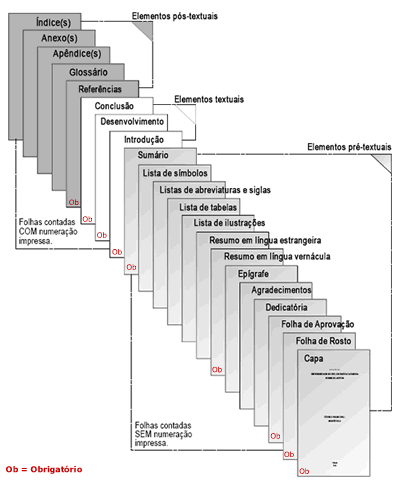
\includegraphics[width=0.6\textwidth]{./04-figuras/abnt}
    \label{fig:ilustfig2}
\end{figure}
\vspace*{-0,9cm}
{\raggedright \fonte{Disponível em: <https://www.intelligentsia.zip.net/estruturamonografia>. Acesso em: 15 ago. 2014.}}\\

Os elementos pré-textuais são compostos de estruturas
obrigatórias: Capa, Folha de ros-to, Folha de aprovação e Sumário. E estruturas opcionais: Lombada, Errata, Dedicatória, Agra-decimentos, Epígrafe, Resumo na língua vernácula, Resumo em língua estrangeira, Lista de ilustrações, Lista de abreviaturas e siglas e Lista de símbolos.

Os elementos textuais são compostos de Introdução,
Desenvolvimento e Conclusão. Os elementos pós-textuais podem é obrigatórios usar as Referências.  E são elementos opcionais: Glossário, Apêndice, Anexo e Índice.

\section{ELEMENTOS PRÉ-TEXTUAIS}

\subsection{Capa}

Elemento obrigatório, sobre o qual se imprimem as informações
indispensáveis à indica-ção do trabalho, na seguinte ordem: nome completo do aluno, título do trabalho, subtítulo se houver, cidade da instituição onde o documento deve ser apresentado, ano de depósito (data da entrega).

\subsection{Lombada}

Elemento opcional, onde as informações devem ser impressas
conforme a norma NBR 12225: nome do autor, impresso longitudinalmente e legível do alto para o pé da lombada. Esta forma possibilita a leitura quando o trabalho está no sentido horizontal, com a face voltada para cima; título do trabalho, impresso da mesma forma que o nome do autor. Elementos alfanuméri-cos de identificação, por exemplo: v. 3.

\subsection{Folha de Rosto}

O anverso da folha de rosto deve conter os elementos na seguinte
ordem: nome completo do aluno, título do trabalho, subtítulo se houver, natureza do trabalho e objetivo (grau pretendi-do), nome da instituição a que é submetido, área de concentração, nome do orientador, local da instituição onde deve ser apresentado, ano de entrega.

\subsection{Errata}

A errata consiste em uma lista das folhas e linhas em que ocorrem
erros, seguida das de-vidas correções. Deve ser inserida após a folha de rosto.

\subsection{Folha de aprovação}

Elemento obrigatório, a folha de aprovação deve conter: nome do
autor, título por exten-so, subtítulo, local e data de aprovação, nome, assinatura e instituição dos membros componen-tes da banca examinadora.

\subsection{Dedicatória}

Folha opcional, onde o aluno presta homenagem ou dedica seu trabalho.

\subsection{Agradecimentos}

Folha opcional, dirigida àqueles que contribuíram para a
elaboração do trabalho.

\subsection{Epígrafe}

Elemento opcional, onde o aluno apresenta uma citação, seguida da
indicação de autoria, relacionada com a matéria tratada no corpo do trabalho. As epígrafes também podem ser apre-sentadas nas folhas de abertura das seções primárias.

\subsection{Resumo}

Consiste na apresentação concisa dos pontos principais de um
texto. Devem ser apresen-tados, de forma clara, os objetivos, o desenvolvimento e as conclusões. Constitui-se em uma sequência de frases objetivas e não uma simples enumeração de tópicos. Deve ser seguido das palavras representativas do conteúdo do trabalho, isto é, palavras-chave e/ou descritores.

\subsection{Abstract}

Consiste em uma versão do resumo em idioma de divulgação
internacional. Deve ser se-guido das palavras representativas do conteúdo do trabalho, isto é, palavras-chave e/ou uniter-mos, na língua.

\subsection{Lista de ilustrações}

As ilustrações (figuras, quadros, tabelas, gráficos) devem ser
numeradas na ordem em que aparecem no texto. É recomendável que sejam feitas listas separadas para cada tipo de ilus-tração. Em cada lista devem constar: número, título e página. Quando as ilustrações forem em grande número e/ou em tamanho maior, podem ser agrupadas no final do trabalho como apên-dice. As ilustrações, com exceção de tabelas, quadros e gráficos, podem ser sinalizadas no texto ou entre parênteses no final da frase, com o termo Figura.

\subsection{Lista de abreviatura e siglas}

Consiste na relação alfabética das abreviaturas e siglas
utilizadas no texto, seguidas das palavras ou expressões correspondentes grafadas por extenso. Recomenda-se a elaboração de lista própria para cada tipo.

\subsection{Lista de símbolos}

Os símbolos devem ser apresentados na lista na ordem em que
aparecem no texto, com o devido significado.

\subsection{Sumário}

Consiste na enumeração das principais divisões, seções e outras
partes do trabalho, na ordem em que aparecem no texto, acompanhadas da página inicial. As divisões devem estar numeradas em algarismos arábicos, a partir da Introdução até às Referências. Havendo subdivi-sões, deve ser adotada a numeração progressiva, sempre em número arábico e a distinção de caracteres, de acordo com a NBR-6027.

\section{ELEMENTOS TEXTUAIS}

\subsection{Introdução}

É a parte inicial do texto onde devem constar a delimitação do
assunto tratado, os objeti-vos da pesquisa e os outros elementos necessários para situar o tema do trabalho.

\subsection{Desenvolvimento}

Parte do texto que contém a exposição ordenada e pormenorizada do
assunto. Divide-se em seções e subseções, que variam em função da abordagem do tema e do método.

\subsection{Conclusão}

Final do texto na qual se apresentam as conclusões correspondentes aos objetivos ou hipóteses.

\section{ELEMENTOS PÓS-TEXTUAIS}

\subsection{Referencias}

É o conjunto padronizado de elementos descritivos, retirados de
um documento, que permite a sua identificação individual. Denomina-se ainda de Referências a lista composta de documentos padronizados e utilizados na elaboração de um trabalho acadêmico.

\subsection{Apêndice}

Consiste em um texto ou um documento elaborado pelo autor, a fim
de complementar sua argumentação, sem prejuízo da unidade nuclear do trabalho. Os apêndices são identificados por letras maiúsculas consecutivas, travessão e pelos respectivos títulos.

\subsection{Anexo}

Consiste em um texto ou documento não elaborado pelo autor, que
serve de fundamen-tação, comprovação e ilustração. Os anexos são identificados por letras maiúsculas consecuti-vas, travessão e pelos respectivos títulos.

\subsection{Índice}

Elemento opcional, elaborado conforme a NBR 6034.

  			% Estrutura    
    %
% Documento: Ilustração
%

\chapter{ILUSTRAÇÕES}

A apresentação de quadros e tabelas está regida pelas Normas de Apresentação Tabular do Instituto Brasileiro de Geografia e Estatística.

\section{FIGURAS}

São desenhos, fotografias, organogramas, esquemas etc. com os respectivos títulos pre-cedidos da palavra Figura e do número de ordem em algarismo arábico.

\begin{figure}[H]
    \centering
    \caption{Exemplo de figura}
	\vspace*{0,2cm}
    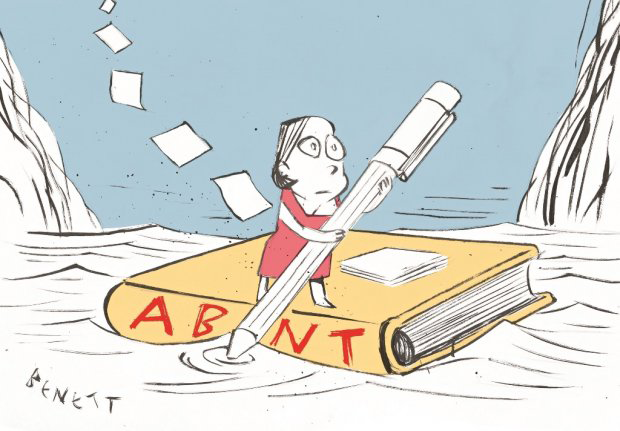
\includegraphics[width=0.8\textwidth]{./04-figuras/navegar_abnt}
    \label{fig:ilustfig}
\end{figure}
\vspace*{-0,9cm}
{\raggedright \fonte{Disponível em: <https://www.gazetadopovo.com.br/abntemfoco>. Acesso em: 24 de jan. de 2015.}}\\

Os títulos devem ser colocados acima das figuras. No texto devem
ser indicados pela pa-lavra Figura acompanhada do número de ordem. E abaixo deve ser indicada sua fonte.

\section{QUADROS}

Denomina-se quadro a apresentação de dados de forma organizada, para cuja compreen-são não seria necessário qualquer elaboração matemático-estatística. A identificação se fará com o nome do elemento Quadro por extenso, seguido do número de ordem em algarismo arábico. Outros elementos do quadro deverão ser descritos de acordo com o padrão usado para
Apresentação tabular.

\begin{quadro}[H]

	\begin{center}
	\caption{Exemplo para quadro.\label{qua:quaexe}}
		\begin{tabular}{|p{7cm}|p{7cm}|}
			\hline
			("Trabalho Conclusão de Curso")\\
			\hline
		\end{tabular}
	\end{center}
	\vspace*{-0,8cm}

	{\raggedright \fonte{Autor desta monografia, 2015.}}
	
\end{quadro}


\section{TABELAS}

Tabelas são conjuntos de dados numéricos, associados a um
fenômeno, dispostos numa determinada ordem da classificação. Expressam as variações qualitativas e quantitativas de um fenômeno. A finalidade básica da tabela é resumir ou sintetizar dados de maneira a fornecer o máximo de informações num mínimo de espaço.

Na apresentação de uma tabela devem ser levados em consideração
os alguns critérios. Toda tabela deve ter significado próprio, dispensando consultas ao texto. A tabela deve ser colo-cada em posição vertical, para facilitar a leitura dos dados. No caso em que isso seja impossível, deve ser colocada em posição horizontal, com o título voltado para a margem esquerda da folha.

Se a tabela ou quadro não couber em uma página, deve ser
continuado na página seguin-te. Neste caso o final não será delimitado por traço horizontal na parte inferior e o cabeçalho será repetido na página seguinte. No texto devem ser indicadas pela palavra Tabela acompanha-da do número de ordem em algarismo arábico.

\begin{table}[H]
    \centering
    \caption[Exemplo tabela]{Exemplo tabela.\label{tab:exetab}}
    \begin{tabular}{cc}
        \hline
            numeros x & numeros y \\
        \hline
            \vspace*{0,15cm} 1 & 15 \vspace*{0,15cm}\\ \hline
            \vspace*{0,15cm} 3 & 4 \vspace*{0,15cm}\\ \hline
            \vspace*{0,15cm} 5 & 6 \vspace*{0,15cm}\\ \hline
            \vspace*{0,15cm} 7 & 8 \vspace*{0,15cm}\\ \hline
			\vspace*{0,15cm} 9 & 11 \vspace*{0,15cm}\\ \hline
            \vspace*{0,15cm} 13 & 15 \vspace*{0,15cm}\\ \hline
        \hline
    \end{tabular}
\end{table}
\vspace*{-0,9cm}
{\raggedright \fonte{Autor desta monografia, 2014.}}

\section{GRÁFICOS}

Depois de sintetizados em tabelas, os dados podem ser
apresentados em gráficos, com a fi-nalidade de proporcionar ao interessado uma visão rápida do comportamento do fenômeno. Serve para representar qualquer tabela de maneira simples, legível e interessante, tornando cla-ros os fatos que poderiam passar despercebidos em dados apenas tabulados.

O elemento de identificação ordenado do gráfico, ou seja, o
número de ordem do mesmo no trabalho. No texto devem ser indicados pela palavra Gráfico, acompanhada do número de ordem em algarismo arábico.



           	% Ilustrações
    %
% Documento: Citações
%

\chapter{CITAÇÕES}

Citação é a menção, no texto, de uma informação colhida de outra fonte. Pode ser direta, indireta e citação de citação. Apresentadas conforme a ABNT NBR 10520

\section{CITAÇÃO DIRETA}

É a transcrição textual dos conceitos de um autor consultado. Um
exemplo: De acordo com as conclusões de Marshall (1980, p. 249) “da mesma forma que não se pode afirmar se é a lâmina inferior ou superior de uma tesoura que corta uma folha de papel, também não se pode discutir se o valor e os preços são governados pela utilidade ou pelo custo de produção”. 

Citação mais longa deve figurar abaixo do texto, em bloco recuado
– de 4 cm da mar-gem esquerda – com letras tamanho 10, sem aspas.

\section{CITAÇÃO INDIRETA}

É a transcrição livre do texto do autor consultado. As citações
indiretas ou parafraseadas dispensam o uso de aspas duplas e do número de páginas.

A produção acadêmica sobre varejo no Brasil fica muito aquem da
importância do seg-mento na economia (ANGELO; SILVA, 1993). É um exemplo de citação indireta.

\section{CITAÇÃO DE CITAÇÃO}

É citação direta ou indireta de um documento ao qual não se teve
acesso aooriginal. De-ve ser citado em nota de rodapé, sendo obrigatória a indicação da Fonte 10 recuo de 4 cm refe-rência de onde foi extraída a informação. Esse tipo de citação só deve ser utilizado nos casos em que realmente o documento original não pode ser recuperado. 

Exemplo: Enguita (apud SILVA, 1991, p. 21) chegou às mesmas
conclusões. As entida-des coletivas podem ser citadas pelas respectivas siglas, desde que na primeira vez em que fo-rem mencionadas apareçam por extenso. Exemplo: ASSOCIAÇÃO BRASILEIRA DO TRA-BALHADOR - ABT (1985)


            	% Citações
    %
% Documento: Tecnicas de referencia
%

\chapter{TÉCNICAS DE REFERÊNCIAS}

É o conjunto padronizado de elementos descritivos, retirados de um documento, que permite a sua identificação individual. Denomina-se ainda de Referências a lista composta de documentos padronizados e utilizados na elaboração de um trabalho acadêmico.

O texto deve estar com o alinhamento justificado, respeitando a formatação indicada pa-ra o tipo de referência. 

\section{MONOGRAFIA}

Monografia Considerada no Todo (livros, folhetos, dissertações,
teses, dicionários, guias). Exemplos: <SOBRENOME, Nome do Autor>. \textbf{Nome
da obra.} Edição.

\section{LIVROS TENDO A ENTIDADE COMO AUTOR}

<NOME DA ENTIDADE>. \textbf{Nome do livro.} Edição.

\section{DOCUMENTOS ELABORADOS POR VÁRIOS AUTORES}

Documentos elaborados por vários autores, com um responsável
intelectual destacado (organizador, coordenador, editor). Exemplo: <SOBRENOME,
Nome do Autor> (Responsabi-lidade atribuída). \textbf{Nome da obra.} Edição.

\section{DOCUMENTOS SEM AUTOR}

<DOCUMENTO e seus subtítulo, caso exista>. Edição. 

\section{ARTIGO OU MATERIA DE REVISTA}

<SOBRENOME, Nome do Autor>. Titulo da matéria. \textbf{Nome da
revista.} Edição.

\section{DOCUMENTO DE EVENTO}

<NOME DO EVENTO, data e local>. Organizador do Evento. Ano,
pagina dos anais onde se encontra a obra. 

\section{EXEMPLOS PARA CITAÇÕES}

Apenas exemplos \cite{7.1.3-1}. Outro \cite{NBR6023:2000}.\cite{NBR10520:1988}. \cite{7.3.2-2}. \cite{7.4.2.1-3}. \cite{7.4.2.1-2}.\cite{7.4.2.3-5}. \cite{7.4.2.1-4}. 
\cite{7.7.1.2-5}. \cite{7.7.1.2-2}. \cite{7.4.2.3-6}. \cite{8.1.1.5}.
            % Tecnica de referencias 

    % Elementos pós textuais
    \postextual
    %
% Documento: Referências Bibliográficas
%

\bibliography{refbase}    % Geração automática das referências por meio do arquivo 'refbase.bib'
       % Referências
    %
% Documento: Apêndices
%

\begin{apendicesenv}

\chapter{ESPECIFICAÇÕES DOS CASOS DE USO}

\begin{table}[!h]
	\begin{center}
		\caption{Especificação do caso de uso Gerenciar Animais}
		\begin{tabular}{ | l |  p{10cm} |}
			\hline
			Código e Nome do Caso de Uso & CdU001 - Gerenciar Animais \\ \hline
			Ator Primário: & Usuário \\
			Ator Secundário: & Não se aplica \\ \hline
			Fluxo Principal de Eventos & P1. O usuário solicita consultar os animais. \\
						   & P2. O sistema apresenta a tela de animais. (IV003) (A1) (A2) \\
						   & P3. O usuário solicita ver um animal em específico. \\
						   & P4. O sistema apresenta a tela de perfil do animal. (IV006) (A3) (A4)  \\
						   & P5. O caso de uso se encerra. \\ \hline
			Fluxo Alternativo:         & A1.1. Em P2 o usuário insere as informações de um animal no formulário e solicita salvá-las. \\
			A1. Adicionar animal       & A1.2. O sistema salva o animal. \\
						   & A1.3. Retorna ao P2. \\ \hline
			Fluxo Alternativo:         & A2.1. Em P2 o usuário tem a intenção de deletar um animal. \\
			A2. Deletar animal         & A2.2. O sistema apaga o animal selecionado. \\
						   & A2.3. Retorna ao P2. \\ \hline
			Fluxo Alternativo:         & A3.1. Em P4 o usuário decide editar animal. \\
			A3. Editar animal          & A3.2. O sistema apresenta a tela de editar animal. (IV007) \\
						   & A3.3. O usuário insere as novas informações do animal. \\
						   & A3.4. O sistema salva essas informações. \\
						   & A3.5. Retorna ao P4. \\ \hline
			Fluxo Alternativo:         & A4.1. Em P4 o decide adicionar uma nova pesagem do animal. \\
			A4. Adicionar peso         & A4.2. O sistema apresenta a tela de adicionar pesagem. (IV008) \\
						   & A4.3. O usuário insere as novas informações de peso do animal. \\
						   & A4.4. O sistema salva essas informações. \\
						   & A4.3. Retorna ao P4. \\ \hline
			Fluxo Alternativo:         & A5.1. Em P4 o usuário decide consultar detalhes do animal. \\
			A5. Consultar Detalhes     & A5.2. O sistema apresenta a tela de detalhes do animal. \\
						   & A5.3. Retorna ao P4. \\
			\hline
		\end{tabular}
		Fonte: Autoria própria.
	\end{center}
\end{table}

\newpage

\begin{table}[!h]
	\begin{center}
		\caption{Especificação do caso de uso Gerenciar Remédios}
		\begin{tabular}{ | l |  p{10cm} |}
			\hline
			Código e Nome do Caso de Uso & CdU002 - Gerenciar Remédios \\ \hline
			Ator Primário: & Usuário \\
			Ator Secundário: & Não se aplica \\ \hline
			Fluxo Principal de Eventos & P1. O usuário solicita consultar os remédios. \\
						   & P2. O sistema apresenta a tela de remédios. (IV004) (A1) (A2) (A3) \\
						   & P3. O caso de uso se encerra. \\ \hline
			Fluxo Alternativo:         & A1.1. Em P2 o usuário insere as informações de um remédio no formulário e solicita salvá-las. \\
			A1. Adicionar remédio      & A1.2. O sistema salva o remédio. \\
						   & A1.3. Retorna ao P2. \\ \hline
			Fluxo Alternativo:         & A2.1. Em P2 o usuário resolve deletar um remédio. \\
			A2. Deletar remédio        & A2.2. O sistema apaga o remédio selecionado. \\
						   & A2.3. Retorna ao P2. \\ \hline
			Fluxo Alternativo:         & A3.1. Em P2 o usuário decide editar um remédio. \\
			A3. Editar remédio         & A3.2. O sistema apresenta a tela de editar remédio. \\
						   & A3.3. O usuário insere as novas informações do remédio. \\
						   & A3.4. O sistema salva essas informações. \\
						   & A3.5. Retorna ao P2. \\
			\hline
		\end{tabular}
		Fonte: Autoria própria.
	\end{center}
\end{table}

\begin{table}[!h]
	\begin{center}
		\caption{Especificação do caso de uso Visualizar Relatórios}
		\begin{tabular}{ | l |  p{10cm} |}
			\hline
			Código e Nome do Caso de Uso & CdU003 - Visualizar Relatórios \\ \hline
			Ator Primário: & Usuário \\
			Ator Secundário: & Não se aplica \\ \hline
			Fluxo Principal de Eventos & P1. O usuário solicita consultar os relatórios. \\
						   & P2. O sistema apresenta a tela de relatórios da fazenda. \\
						   & P3. O caso de uso se encerra. \\
			\hline
		\end{tabular}
		Fonte: Autoria própria.
	\end{center}
\end{table}

\newpage

\begin{table}[!h]
	\begin{center}
		\caption{Especificação do caso de uso Gerenciar Medicação}
		\begin{tabular}{ | l |  p{10cm} |}
			\hline
			Código e Nome do Caso de Uso & CdU004 - Gerenciar Medicação \\ \hline
			Ator Primário: & Usuário \\
			Ator Secundário: & Não se aplica \\ \hline
			Fluxo Principal de Eventos & P1. O usuário solicita consultar medicação. \\
						   & P2. O sistema apresenta a tela de medicação. (IV005) (A1) (A2) (A3) \\
						   & P3. O caso de uso se encerra. \\ \hline
			Fluxo Alternativo:         & A1.1. Em P2 o usuário insere as informações de uma medicação e solicita salvá-las. \\
			A1. Adicionar medicação    & A1.2. O sistema salva a medicação. \\
						   & A1.3. Retorna ao P2. \\ \hline
			Fluxo Alternativo:         & A1.1. Em P2 o usuário resolve deletar uma medicação. \\
			A2. Deletar medicação      & A2.2. O sistema apaga a medicação selecionada. \\
						   & A2.3. Retorna ao P2. \\ \hline
			Fluxo Alternativo:         & A3.1. Em P2 o usuário decide editar uma medicação. \\
			A3. Editar medicação       & A3.2. O sistema apresenta a tela de editar medicação. \\
						   & A3.3. O usuário insere as novas informações da medicação. \\
						   & A3.4. O sistema salva essas informações. \\
						   & A3.5. Retorna ao P2. \\
			\hline
		\end{tabular}
		Fonte: Autoria própria.
	\end{center}
\end{table}


\chapter{DIAGRAMAS DE ATIVIDADE}
\begin{figure}[H]
	\begin{center}
		\caption{Diagrama da Atividade de Gerenciar Animal parte 1}
		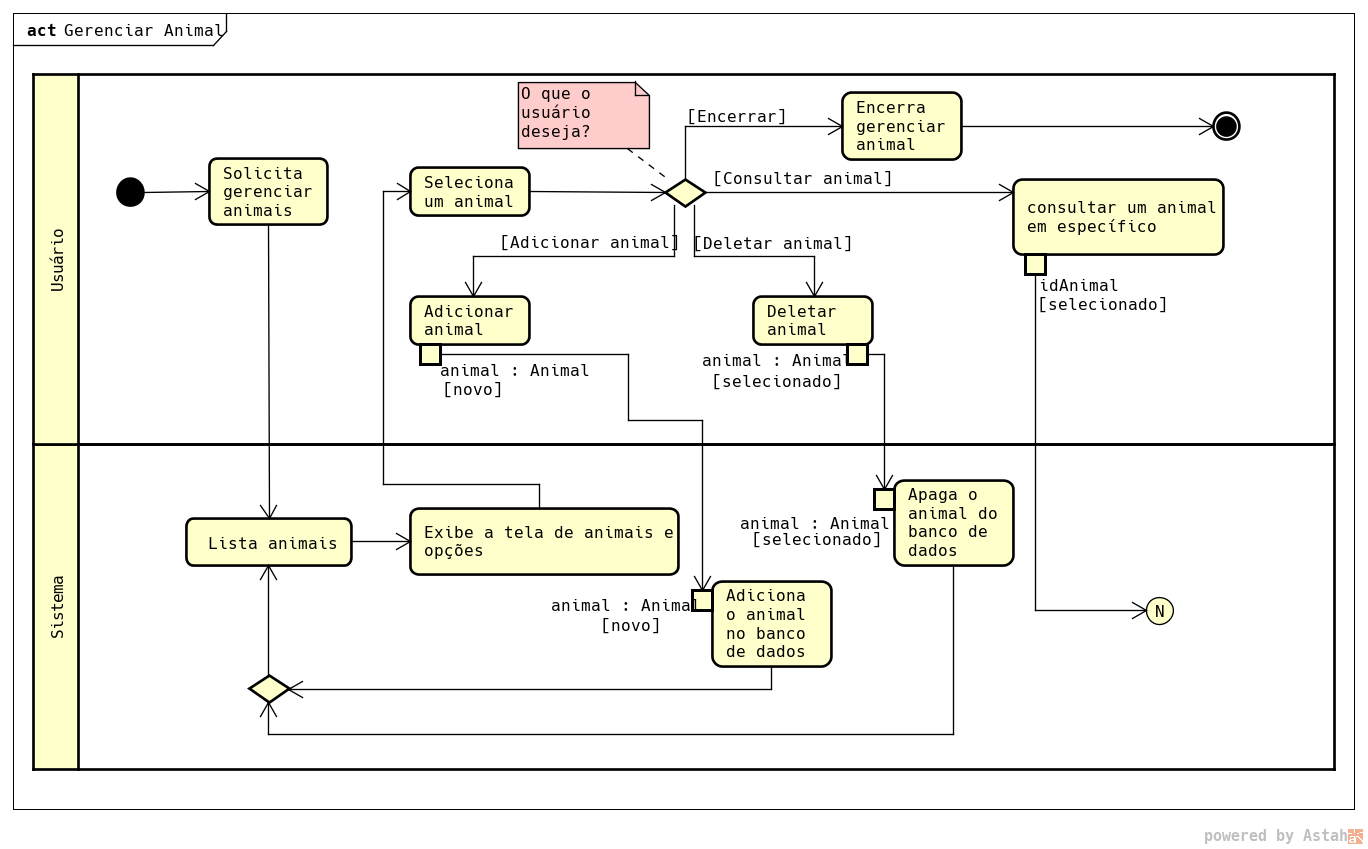
\includegraphics[width=\textwidth]{../img/GerenciarAnimal1.png}

		Fonte: Autoria própria.
	\end{center}
\end{figure}

\begin{figure}[H]
	\begin{center}
		\caption{Diagrama da Atividade de Gerenciar Animal parte 2}
		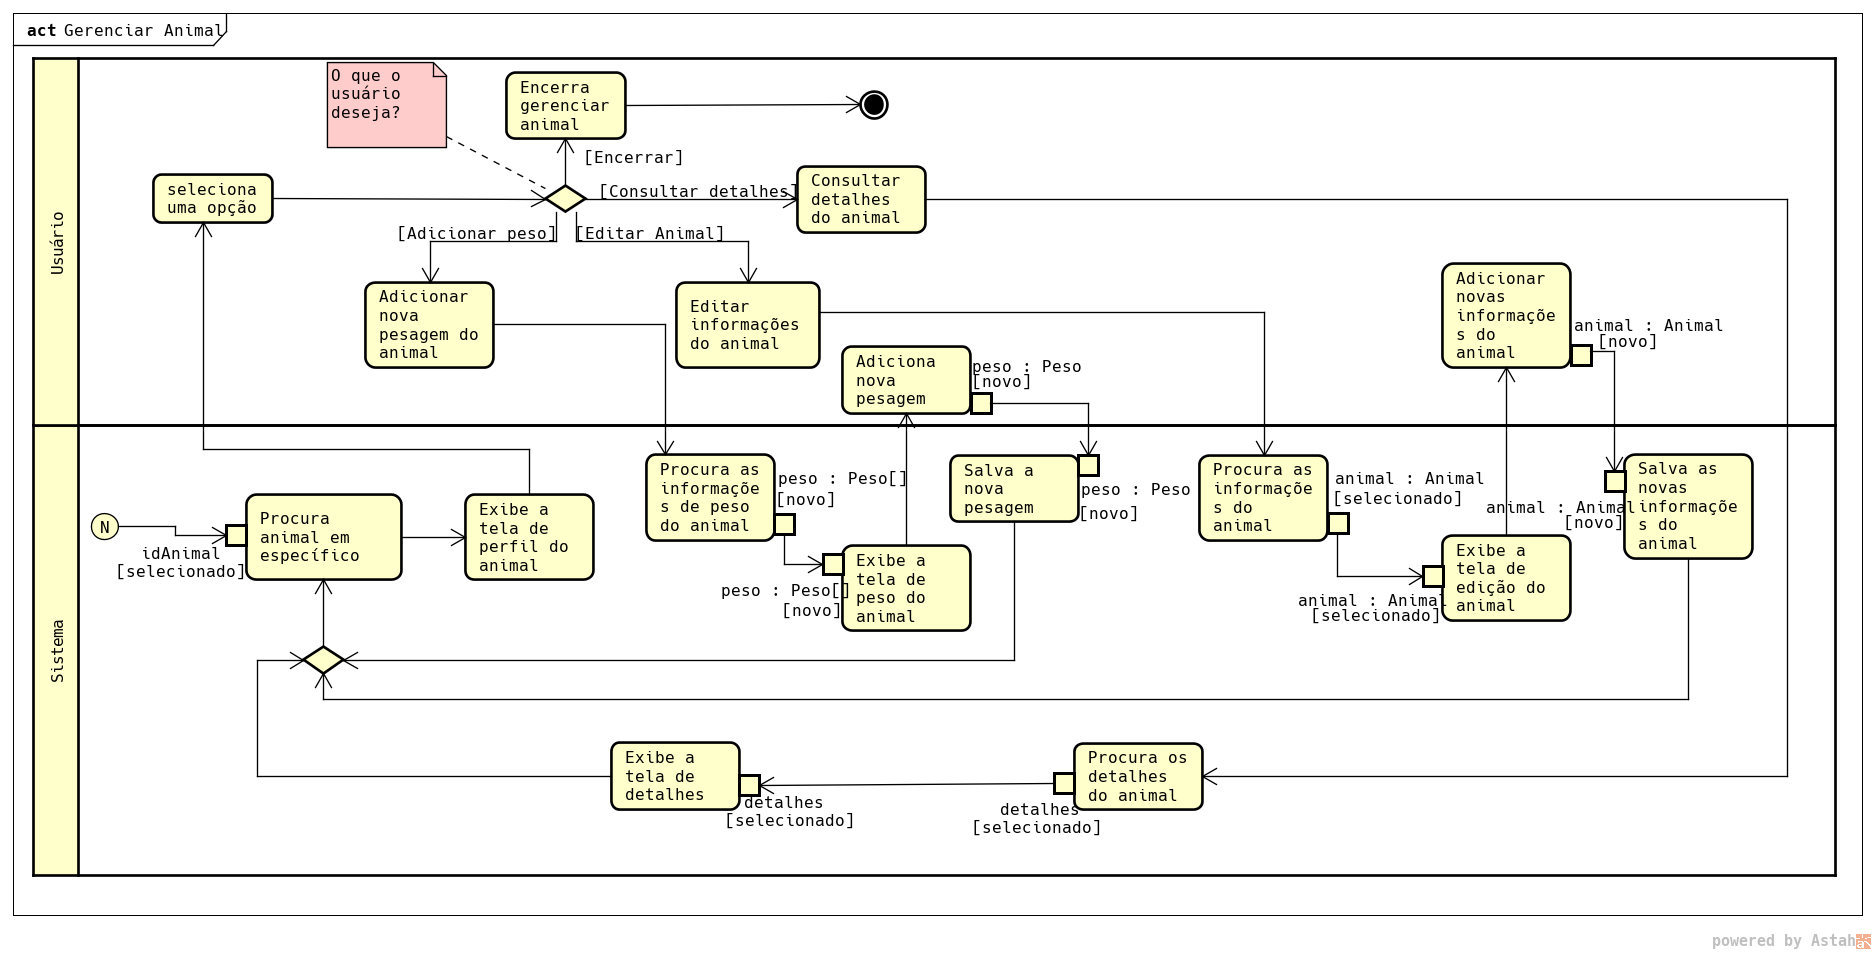
\includegraphics[width=\textwidth]{../img/GerenciarAnimal2.png}

		Fonte: Autoria própria.
	\end{center}
\end{figure}

\begin{figure}[H]
	\begin{center}
		\caption{Diagrama da Atividade de Gerenciar Remédios}
		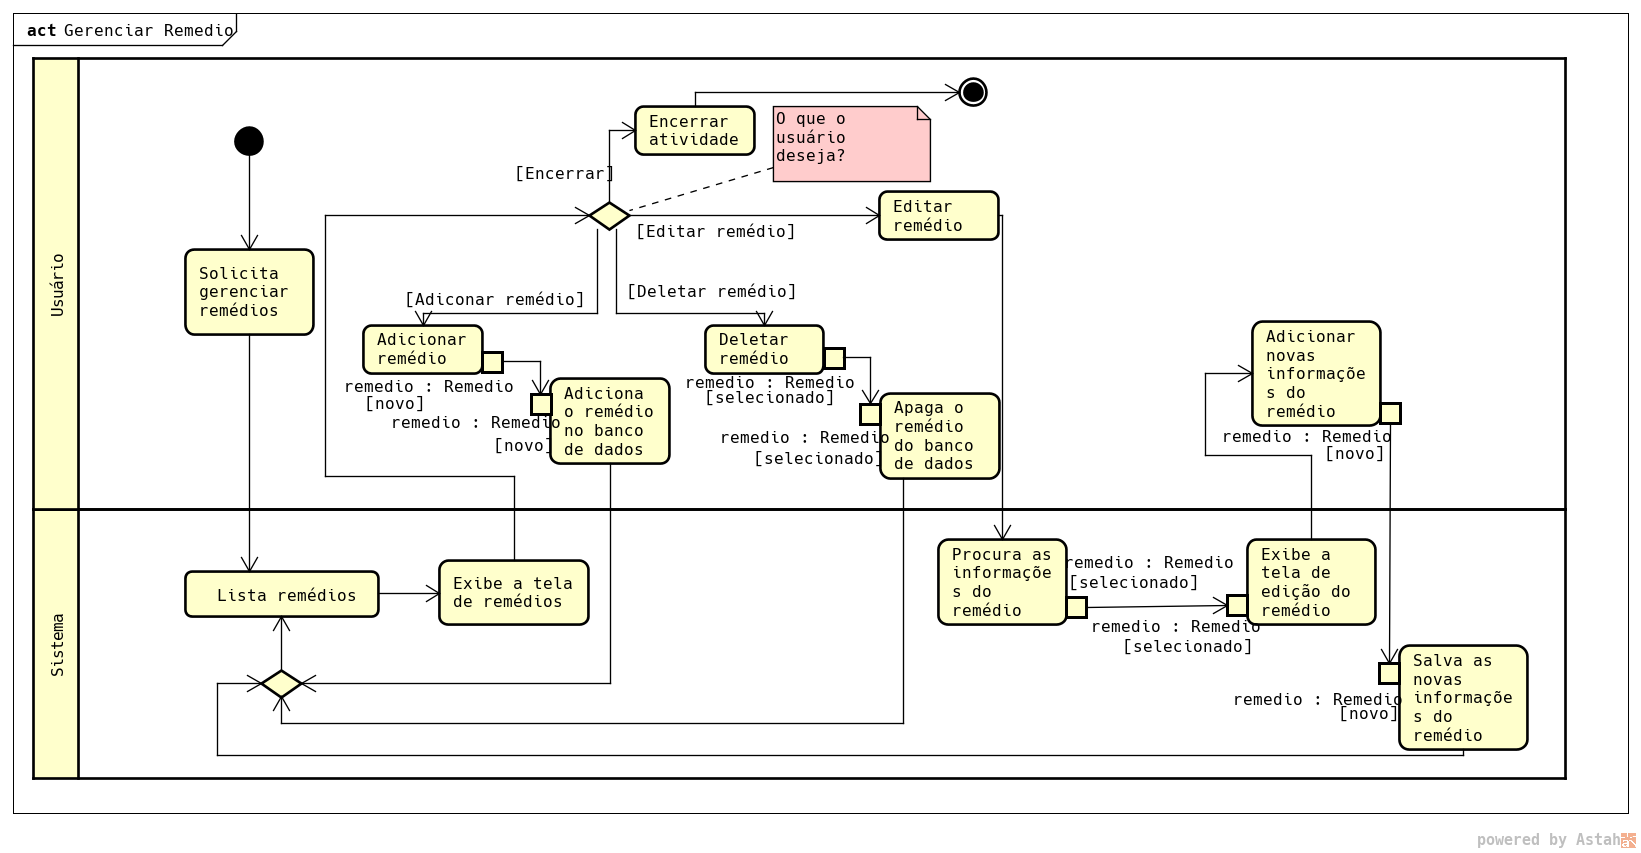
\includegraphics[width=\textwidth]{../img/GerenciarRemedio.png}

		Fonte: Autoria própria.
	\end{center}
\end{figure}

\begin{figure}[H]
	\begin{center}
		\caption{ Diagrama da Atividade de Gerenciar Medicações}
		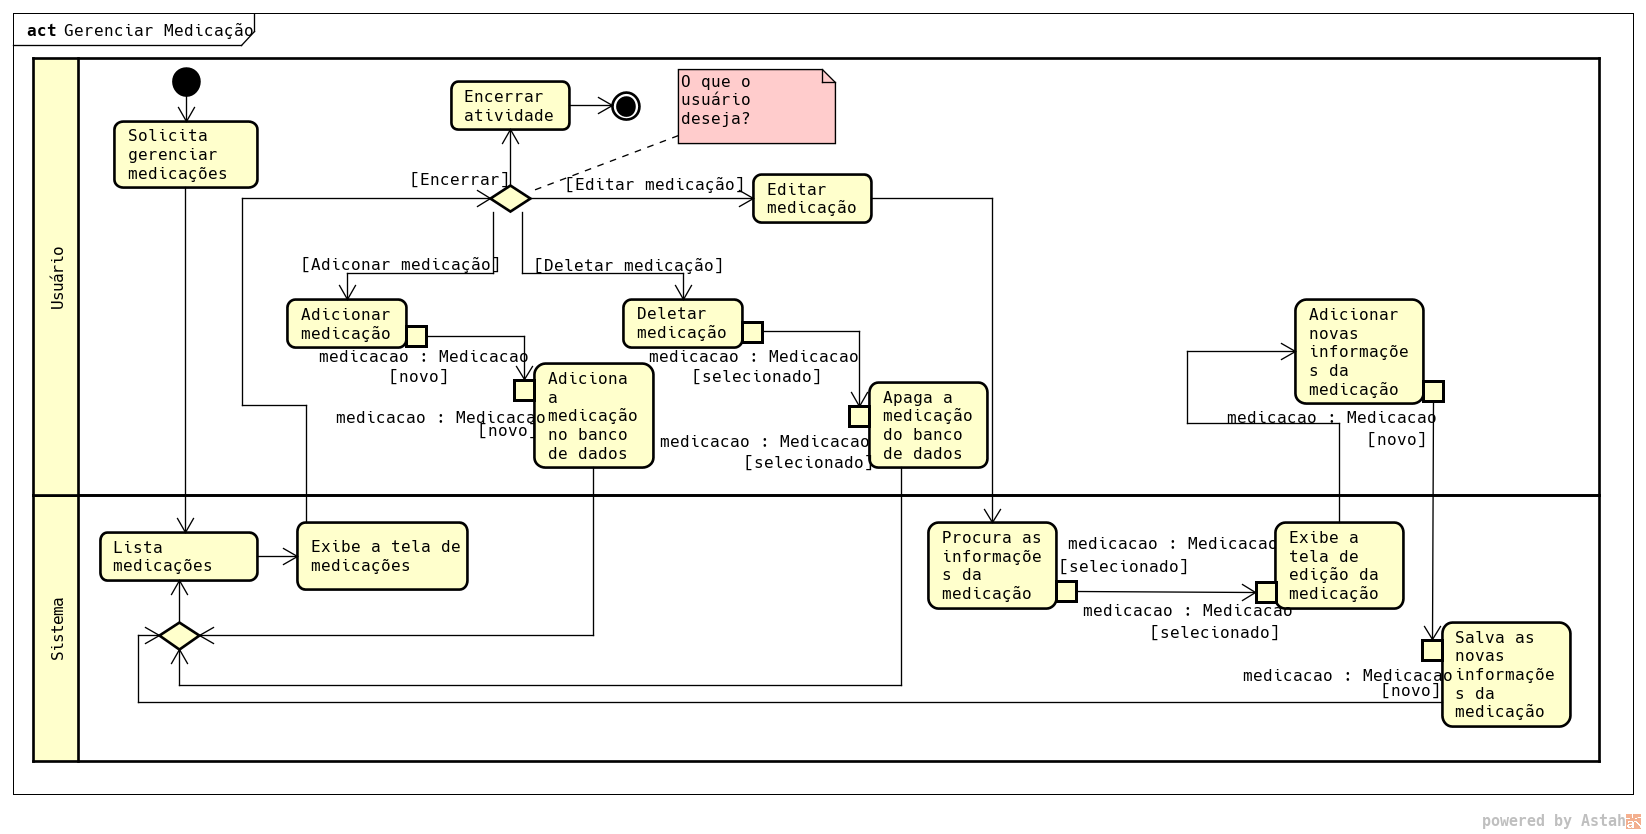
\includegraphics[width=\textwidth]{../img/GerenciarMedicacao.png}

		Fonte: Autoria própria.
	\end{center}
\end{figure}

\begin{figure}[H]
	\begin{center}
		\caption{Diagrama da Atividade de Visualizar Relatórios}
		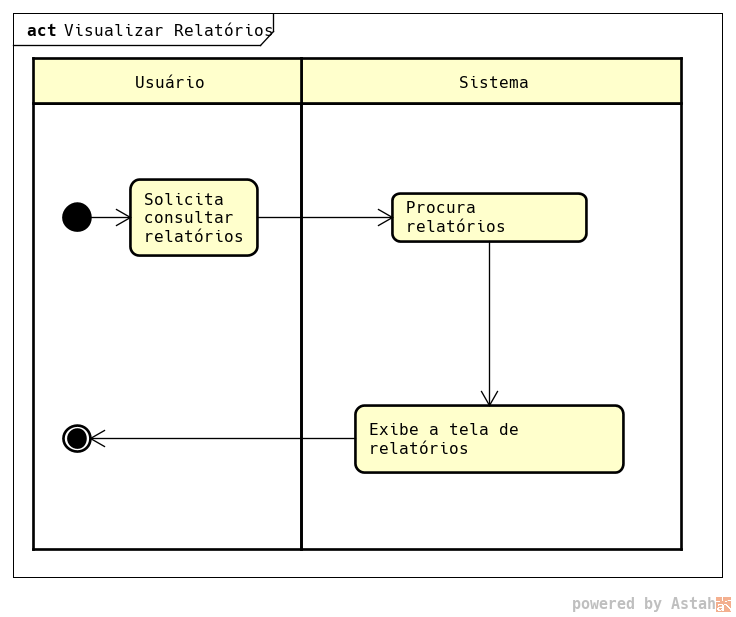
\includegraphics[width=\textwidth]{../img/Relatorios.png}

		Fonte: Autoria própria.
	\end{center}
\end{figure}

\end{apendicesenv}
         % Apêndices
    %
% Documento: Anexos
%

\begin{anexosenv}

\chapter{Como elaborar}

Anexo é texto ou documento não elaborado pelo autor, que serve de fundamentação, comprovação e ilustração. Elemento opcional. Deve ser precedido da palavra ANEXO, identifi-cado por letras maiúsculas consecutivas, travessão e pelo respectivo título. Utilizam-se letras maiúsculas dobradas, na identificação dos anexos, quando esgotadas as letras do alfabeto.


\end{anexosenv}            % Anexos
    %\printindex                                             % Índice remissivo

\end{document}
